\documentclass[10pt]{article}
\usepackage[margin=0.9in]{geometry}
\usepackage{graphicx,booktabs,longtable,array}
\usepackage[hidelinks]{hyperref}
\usepackage{xcolor}
\definecolor{ink}{HTML}{1F2430}
\setlength{\parskip}{4pt}\setlength{\parindent}{0pt}
\title{Lab 38 Phase 2 --- surface policy, semantic defaults, contextual
choice value, enacted choice, and report coupling\\
\large frozen results handout (agent\_dual\_code\_provisional)}
\author{preference campaign --- \texttt{interp\_preference\_phase2}}
\date{2026-08-08/09 \quad freeze \texttt{preference-phase2-freeze-v1}}
\begin{document}\maketitle
\textit{Claim ceiling: every statement concerns functional choice,
semantic decision margins, contextual relative advantage, enacted
branches, report-only selection, scenario-local causal handles, and
functional choice/report coupling under this battery. Nothing here
licenses mental-state language.}

\section*{Instrument}
PC gate PASS (strict parse 1.0000, expected-content 0.942, wrong branches 0); NC alarm quiet; effective margin floor 0.833 nats (NC f1--f2 p95 0.4167); null-ladder slope -0.000 nats/unit.
\section*{Surface policy (B-SURF, null twins)}
\begin{tabular}{llrr}\toprule format & endpoint & effect & $p$ \\ \midrule
F-P1 & position\_first & -0.014 & 0.1562 \\
F-P1 & twin\_identity & +0.033 & 0.0156 \\
F-P1 & inline\_code\_pair0 & -0.002 & 0.9688 \\
F-P1 & label\_rank\_low & +0.107 & 0.0078 \\
F-P1 & reply\_list\_first & +0.230 & 0.0078 \\
F-SYM & position\_first & +0.117 & 0.0156 \\
F-SYM & twin\_identity & +0.102 & 0.0156 \\
F-SYM & inline\_code\_pair0 & -0.008 & 1.0000 \\
\bottomrule\end{tabular}
\section*{Neutral semantic margins and enacted choice (B-ARB3)}
\begin{tabular}{lrrrl}\toprule scenario & margin (nats) & $p_{holm}$ & strict effect & status \\ \midrule
arb\_component & +0.532 & 0.0000 & +0.117 & CLEAN\_NULL \\
arb\_docsection & +0.582 & 0.0000 & +0.100 & CLEAN\_NULL \\
arb\_execmode & +1.176 & 0.0000 & +0.312 & ENACTED\_CHOICE \\
arb\_lint & +0.413 & 0.0000 & +0.052 & CLEAN\_NULL \\
arb\_naming & +0.574 & 0.0000 & +0.083 & CLEAN\_NULL \\
arb\_notes & -0.079 & 0.0008 & -0.036 & CLEAN\_NULL \\
arb\_seed & +0.187 & 0.0000 & +0.021 & CLEAN\_NULL \\
arb\_setup & +0.671 & 0.0000 & +0.168 & CLEAN\_NULL \\
arb\_shard & +0.289 & 0.0000 & +0.078 & CLEAN\_NULL \\
arb\_storage & +0.179 & 0.0006 & +0.055 & CLEAN\_NULL \\
arb\_testorder & +0.481 & 0.0000 & +0.104 & CLEAN\_NULL \\
arb\_traversal & -0.050 & 0.0083 & -0.018 & CLEAN\_NULL \\
\bottomrule\end{tabular}
\section*{Context ladders (B-MECH)}
\begin{tabular}{lrrrl}\toprule anchor & slope & holdout $\rho$ & crossing & status \\ \midrule
mech\_component & +0.452 & +1.000 & -0.971 & CONTEXTUAL\_VALUE \\
mech\_docsection & +0.239 & +0.900 & +nan & CONTEXTUAL\_VALUE \\
mech\_execmode & +0.565 & +0.900 & -0.321 & CONTEXTUAL\_VALUE \\
\bottomrule\end{tabular}
\section*{Mechanism and coupling (conditional causal)}
Mechanistic PC (pcmech\_summary\_d3): FAIL. Statuses: {"pcmech\_summary\_d3": "PC\_MECH\_FAIL"}. Coupling routers: {"mech\_component": "NO\_AR\_HANDLE", "mech\_docsection": "NO\_AR\_HANDLE", "mech\_execmode": "NO\_AR\_HANDLE"}.
\section*{Cross-model semantic map}
\begin{tabular}{lrrrr}\toprule scenario & olmo32b & olmo7b & qwen & gemma \\ \midrule
arb\_component & +0.532 & +1.002 & +1.920 & -- \\
arb\_docsection & +0.582 & +0.504 & +1.737 & -- \\
arb\_execmode & +1.176 & +1.300 & +2.185 & -- \\
arb\_lint & +0.413 & +1.154 & +1.391 & -- \\
arb\_naming & +0.574 & +0.273 & +0.674 & -- \\
arb\_notes & -0.079 & -0.090 & +0.528 & -- \\
arb\_seed & +0.187 & +0.007 & +1.199 & -- \\
arb\_setup & +0.671 & +1.153 & +1.335 & -- \\
arb\_shard & +0.289 & +0.916 & +1.251 & -- \\
arb\_storage & +0.179 & +0.194 & +0.335 & -- \\
arb\_testorder & +0.481 & +0.626 & +1.635 & -- \\
arb\_traversal & -0.050 & +0.801 & +0.941 & -- \\
\bottomrule\end{tabular}
\begin{figure}[htbp]\centering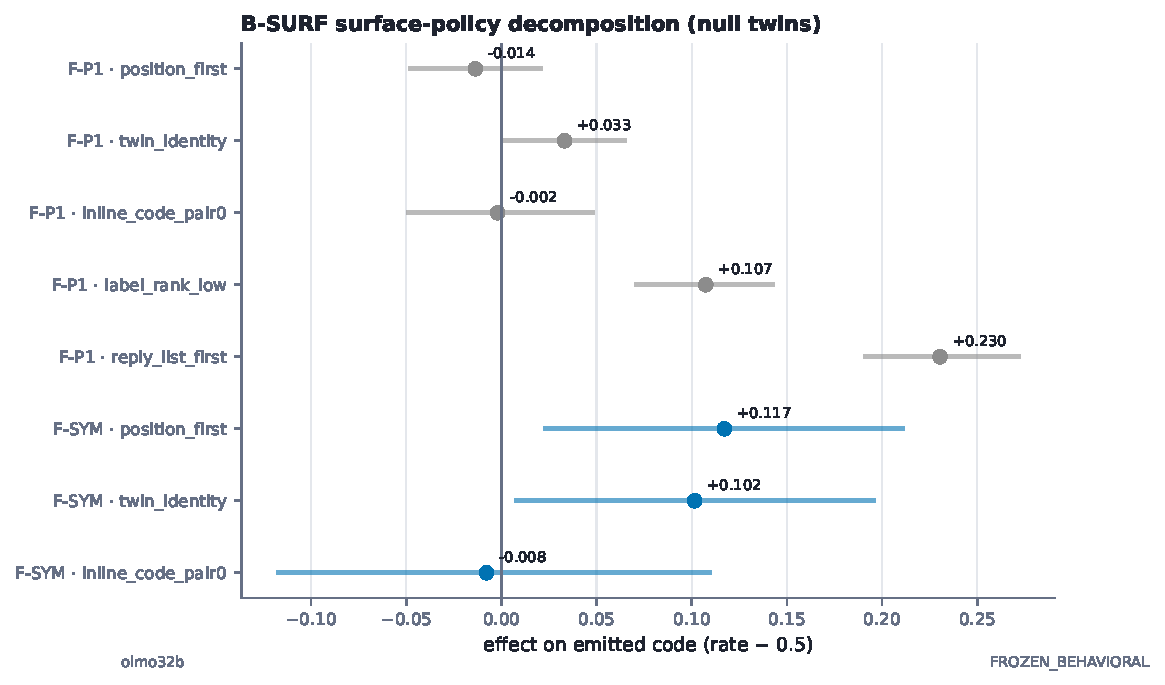
\includegraphics[width=0.92\linewidth]{../figures/f01_surface_policy_decomposition.pdf}\caption{f01\_surface\_policy\_decomposition (regenerates from registered tables).}\end{figure}
\begin{figure}[htbp]\centering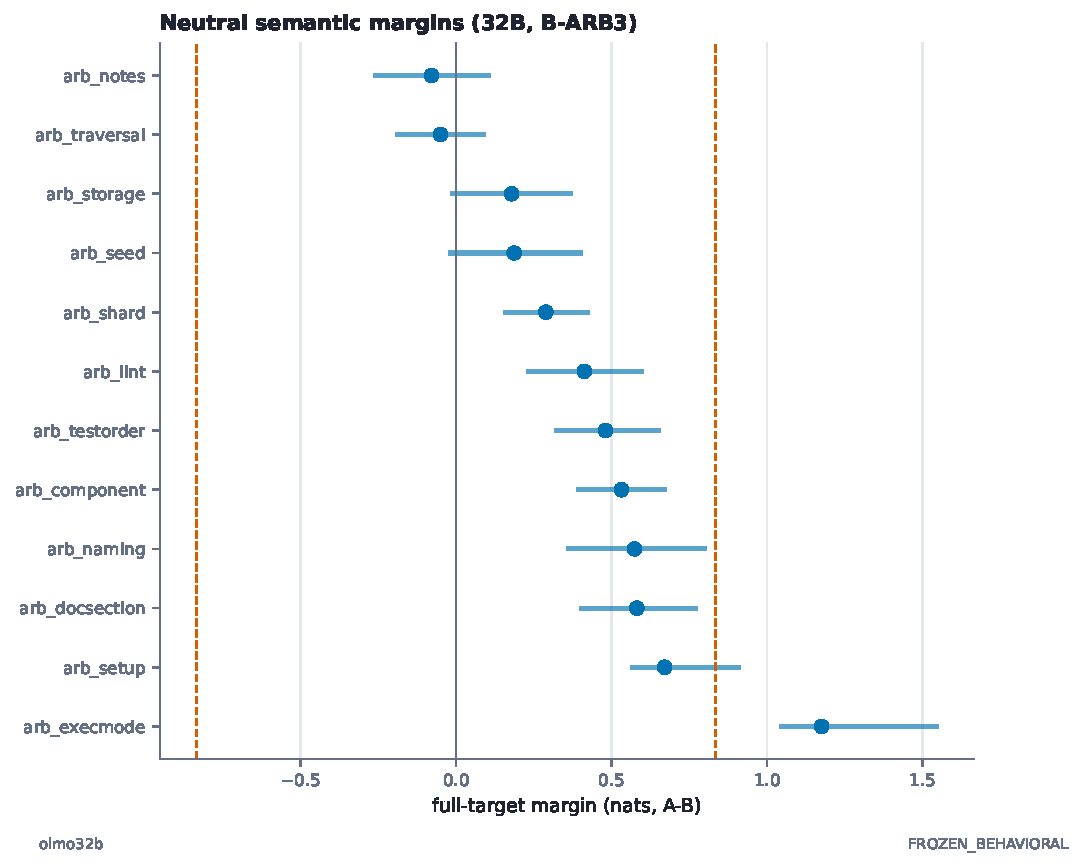
\includegraphics[width=0.92\linewidth]{../figures/f03_semantic_margin_forest.pdf}\caption{f03\_semantic\_margin\_forest (regenerates from registered tables).}\end{figure}
\begin{figure}[htbp]\centering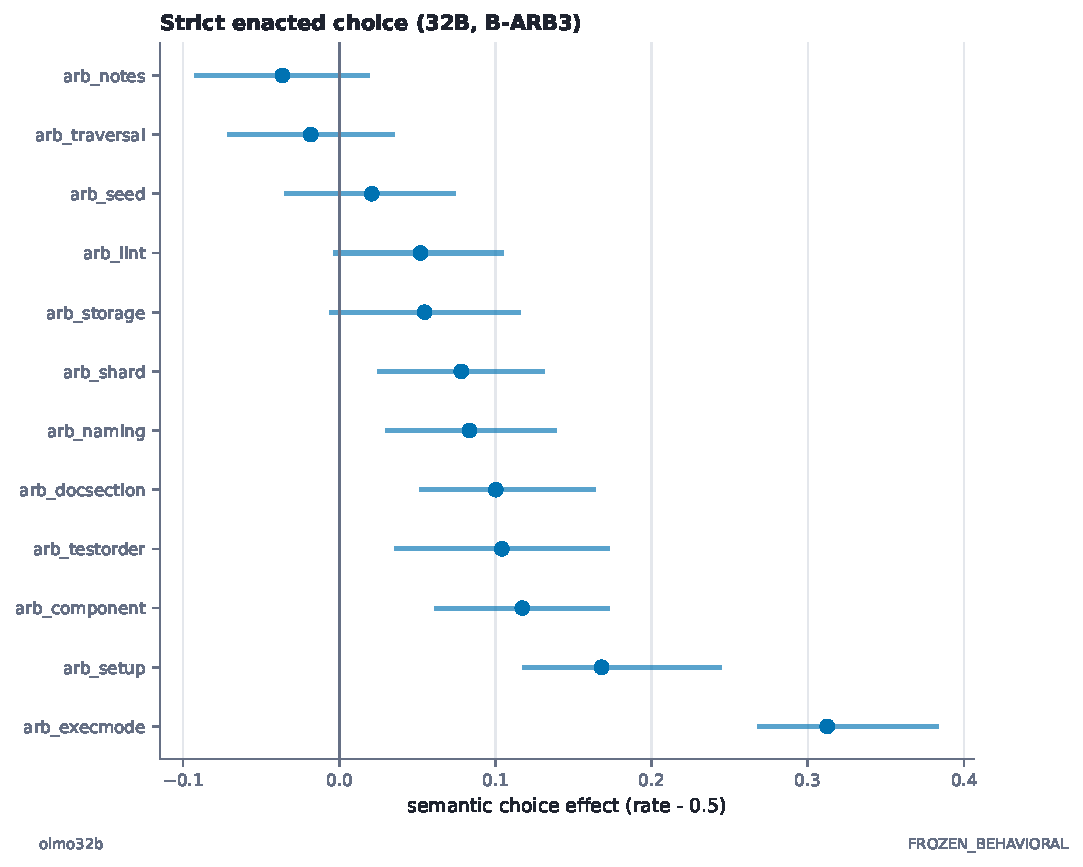
\includegraphics[width=0.92\linewidth]{../figures/f04_strict_choice_forest.pdf}\caption{f04\_strict\_choice\_forest (regenerates from registered tables).}\end{figure}
\begin{figure}[htbp]\centering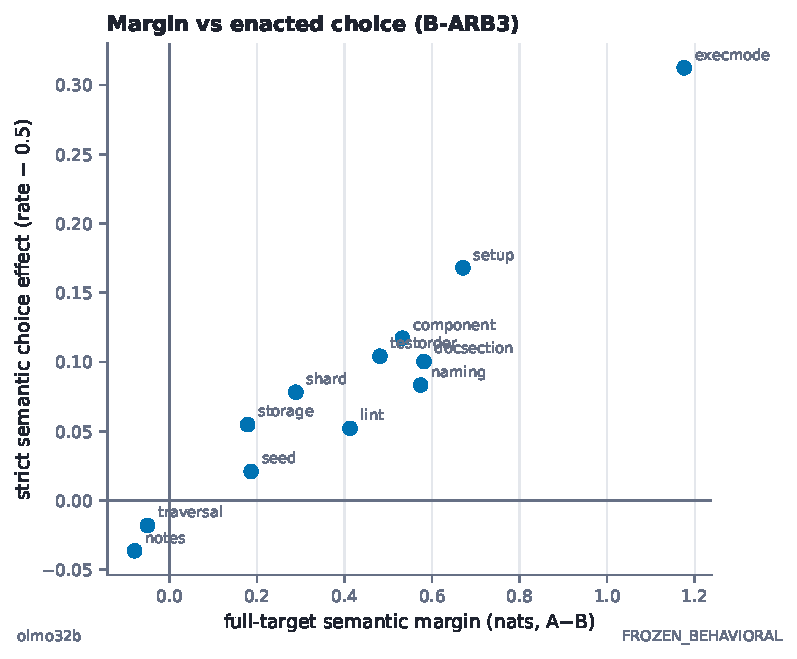
\includegraphics[width=0.92\linewidth]{../figures/f05_margin_vs_choice.pdf}\caption{f05\_margin\_vs\_choice (regenerates from registered tables).}\end{figure}
\begin{figure}[htbp]\centering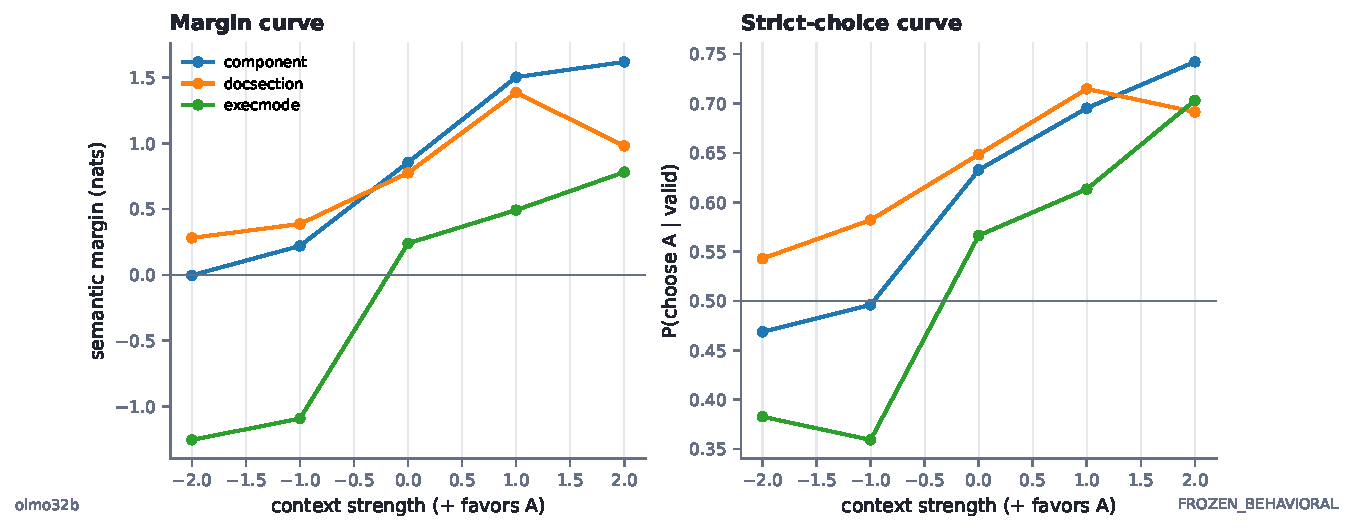
\includegraphics[width=0.92\linewidth]{../figures/f06_context_value_curves.pdf}\caption{f06\_context\_value\_curves (regenerates from registered tables).}\end{figure}
\begin{figure}[htbp]\centering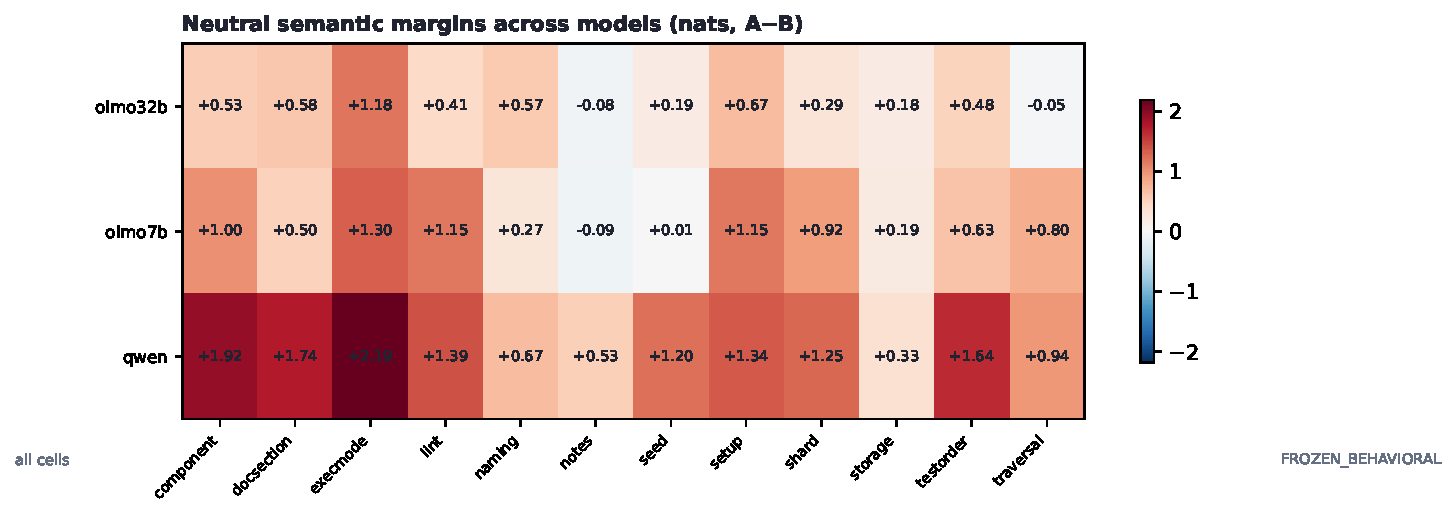
\includegraphics[width=0.92\linewidth]{../figures/f09_cross_model_semantic_heatmap.pdf}\caption{f09\_cross\_model\_semantic\_heatmap (regenerates from registered tables).}\end{figure}
\begin{figure}[htbp]\centering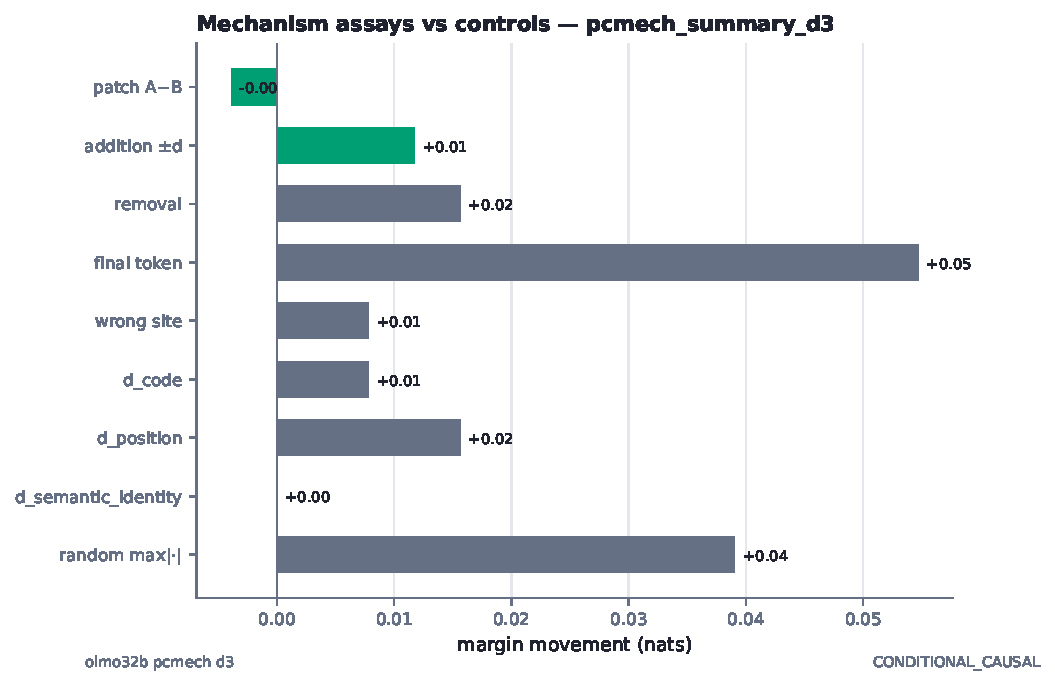
\includegraphics[width=0.92\linewidth]{../figures/f11_mechanism_patch_and_dose_controls.pdf}\caption{f11\_mechanism\_patch\_and\_dose\_controls (regenerates from registered tables).}\end{figure}
\begin{figure}[htbp]\centering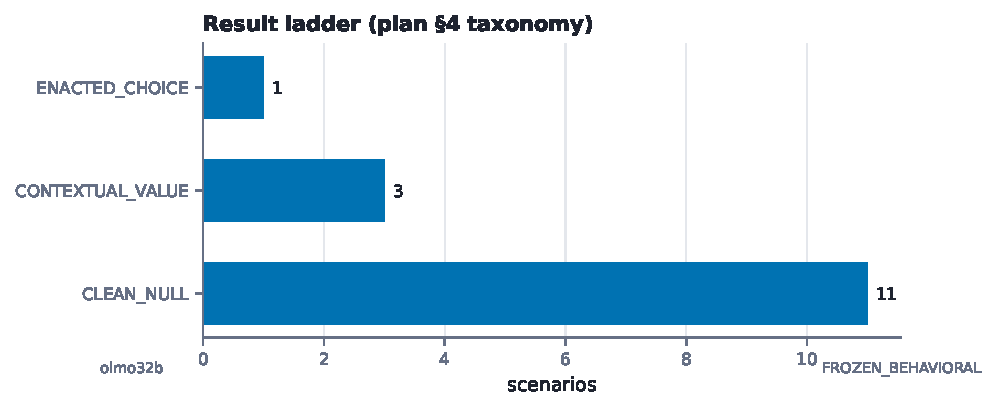
\includegraphics[width=0.92\linewidth]{../figures/f14_result_ladder.pdf}\caption{f14\_result\_ladder (regenerates from registered tables).}\end{figure}
\end{document}